
\section{De kostenfunctie}

Een groot deel van machine learning, zeker wanneer we het hebben over \textit{gecontroleerd leren}, heeft betrekking op het voorspellen van de waarde van een variabele op basis van de waarde van een andere variabele. Stel je bijvoorbeeld voor dat we de verkoopwaarde van een huis willen voorspellen. Vanzelfsprekend zijn er legio aspecten die hierbij een rol spelen, maar een eerste eigenschap waar we naar zouden kunnen kijken is de grootte van het huis in kwestie. De vraag wordt dan of we op basis van de grootte van het huis iets kunnen zeggen over de waarde hiervan.

Overigens raken we hier direct aan een aardig aspect van \textit{machine learning}, namelijk dat twee of meer variabelen prima een gelijk verloop kunnen vertonen, zonder dat hier een causaal verband tussen bestaat. Wanneer je aspecten van je data met elkaar in verband wilt brengen, moet je je er dus altijd van vergewissen dat hier een \textit{logische} verhouding tussen bestaat. Je loopt anders het risico op zogenaamde \textit{spurieuze verhoudingen}. Zie voor mooie voorbeelden hiervan \url{http://tylervigen.com/spurious-correlations}.

\subsection{De som van de gekwadrateerde afwijking}
Wanneer we de verhouding tussen de grootte van een huis plotten tegenover de waarde van datzelfde huis, krijgen we bijvoorbeeld een plaatje als in figuur \ref{img:scatter}:

\begin{figure}[h]
\centering
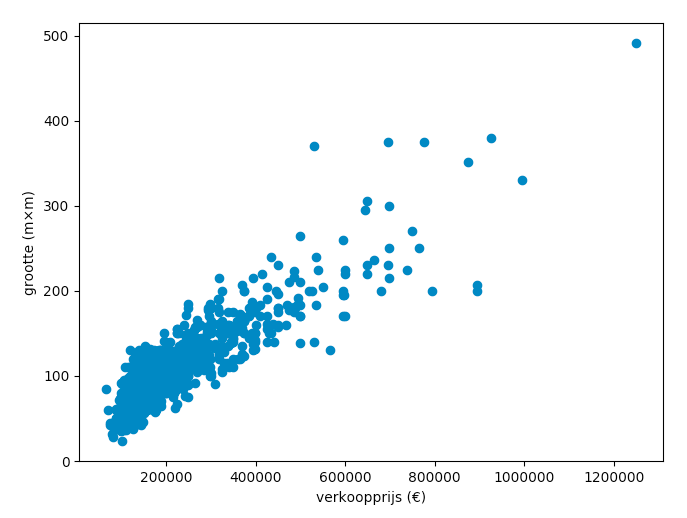
\includegraphics[width=.75\textwidth]{scatter1}
\caption{Scatterplot van de grootte van een huis ten opzichte van de prijs.\label{img:scatter}}
\end{figure}

De scatterplot in figuur \ref{img:scatter} toont een aantal \textit{observaties}: elk punt $(x,y)$ is een observatie van de prijs en de grootte van een huis. Zoals je ziet, is er wel een bepaalde correlatie tussen deze twee grootheden te identificeren: hoe groter het huis, hoe duurder. De vraag is nu hoe exact deze verhouding is.

Om de manier waarop je deze vraag kunt beantwoorden te verduidelijken, gebruiken we de wat eenvoudiger scatterplot in figuur \ref{img:scatter2}. Hier zijn twee variabelen $x$ en $y$ tegenover elkaar gezet, met daarin vier observaties: $p^{(1)}=(1,1)$, $p^{(2)}=(1,4)$, $p^{(3)}=(3,4)$ en $p^{(4)}=(4,4)$. Verder stellen we als \textit{hypothese} dat de waarde van $y$ gelijk is aan de waarde van $x$, kortom dat $y=x$. Deze hypothese wordt in figuur \ref{img:scatter2} door de dunne rode lijn weergegeven.

\begin{figure}[h]
\centering
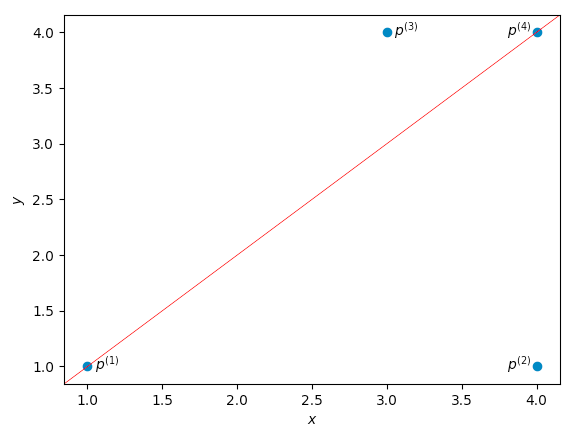
\includegraphics[width=.75\textwidth]{scatter2}
\caption{Eenvoudige scatterplot met vier observaties.\label{img:scatter2}}
\end{figure}

Uitgaande van deze hypothese blijkt dat de punten $p^{(1)}$ en $p^{(4)}$ exact aan de voorspelde waarde voldoen, maar twee punten ook niet. Voor punt $p^{(2)}$ is de voorspelde waarde 4, maar de werkelijke waarde is 1; voor punt $p^{(3)}$ is de voorspelde waarde 3, maar is de werkelijke waarde 4. Het verschil tussen de voorspelde en de werkelijke waarde is dus $-3$ en $1$ (zie figuur \ref{img:scatter3}).

\begin{figure}[h]
\centering
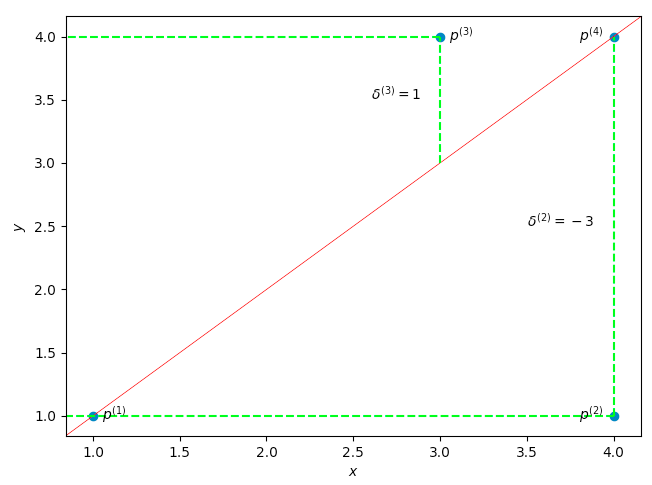
\includegraphics[width=.75\textwidth]{scatter3}
\caption{Het verschil tussen voorspelde en actuele waarden.\label{img:scatter3}}
\end{figure}

Wanneer we nu willen bepalen hoe goed onze hypothese is, moeten we al deze verschillen tussen de voorspelde en werkelijke waarde met elkaar optellen. Een probleem hierbij is echter dat deze verschillen zowel positief als negatief kunnen zijn. Hierdoor zou de som van al deze verschillen lager kunnen uitpakken dan werkelijk het geval is: zo is in het voorbeeld in figuur \ref{img:scatter3} de som van alle verschillen gelijk aan $1+-3=2$, terwijl we intuïtief aanvoelen dat deze som eerder $1+3=4$ zou moeten zijn.

Om dit probleem te adresseren tellen we de \textit{kwadraten} van al deze verschillen bij elkaar op, zodat ook negatieve verschillen een positieve bijdrage leveren. Om te bepalen hoe goed de hypothese is, delen we tenslotte deze som door het aantal datapunten, zodat we een \textit{gemiddelde afwijking} krijgen. Deze afwijking vormt de \textit{kost} van onze hypothese: feitelijk beschrijft dit wat het kost om met een bepaalde hypothese een set van datapunten te beschrijven. Hoe lager deze kosten hoe beter de hypothese is.

\[
\begin{aligned}
KOST &= \frac{0^2 + (-3)^2 + 1^2 + 0^2}{4}\\
&= \frac{0+9+1+0}{4}=2,5
\end{aligned}
\]


\subsection{Gegevensnotatie}
Om hier goed over te kunnen redeneren en mee te kunnen rekenen is een conventie nodig met betrekking tot de notatie van de verschillende elementen.

In het voorbeeld hierboven is steeds gesproken over slechts één eigenschap waar naar gekeken wordt om de prijs van een huis te bepalen: de grootte van het woonoppervlak. In werkelijkheid zijn meestal meer eigenschappen van data die je in je berekeningen mee wilt nemen. Deze eigenschappen (Engels: \textit{features}) worden weergegeven door middel van een subscript $j$. De individuele observaties (\textit{samples}) $x$ uit de volledige trainingsdata $X$ worden beschreven met een superscript $i$ tussen haakjes. Dus $x_4^{(2)}$ heeft betrekking op de waarde van de \textit{vierde} eigenschap van het \textit{tweede} observatie. Stel je voor dat de trainingsdata bestaat uit vier eigenschappen, dan geldt dus:

\[
x^{(i)}  = 
\begin{bmatrix}
x_1^{(i)} & x_2^{(i)} & x_3^{(i)} & x_4^{(i)}
\end{bmatrix} \in X.
\]

Het totaal aantal observaties in de trainingsdata wordt weergegeven met $m$ en de verwachte uitkomst met $y$. Voor elk sample $x^{(i)} \in X$ (waarvoor geldt $1 \le i \le m$) is er een corresponderende waarde $y^{(i)}$.

De hypothese $h$ die we formuleren geeft als het ware een gewicht aan alle eigenschappen (\textit{features}) van de trainingsset. Deze gewichten worden weergeven met de Griekse kleine letter theta, $\theta$, met een subscript om aan te geven bij welke eigenschap dat specifieke gewicht hoort. Het aantal eigenschappen van een dataset wordt aangegeven met $n$, dus $\theta$ is een $n \times 1$ kolomvector. Aan deze vector wordt meestal nog een initiële waarde $\theta_0$ toegevoegd (zoals de algemene formule van een lijn: $y=b+ax$).

\[
\theta=
\begin{bmatrix}
\theta_1 \\
\theta_2 \\
\theta_3 \\
\vdots \\
\theta_n \\
\end{bmatrix}
\]



In het huizen-voorbeeld is er maar één eigenschap waar naar gekeken wordt, dus de hypothese is in dit geval $h(x) = \theta_0 + \theta_1x$. In de grafiek in figuur \ref{img:scatter4} is een aantal hypothesen met verschillende waarden voor $\theta$ getekend. Elk van deze lijnen correspondeert met een bepaalde hypothese over $y$ gegeven $x$ en een bepaalde waarde van $\theta$. Meer in het algemeen zijn deze hypothesen dus functies van $x$ die afhankelijk zijn van specifieke waarden van $\theta_0$ en $\theta_1$. Zo is lijn 1 in de grafiek gegeven door $h_\theta(x)=0,5+2x$, lijn 2 door $h_\theta(x)=2$ en lijn 3 door $h_\theta(x)=0,5x$. De hypothese, kortom, van de waarde van $y$ is gelijk aan elke waarde van $\theta$ vermenigvuldigd met de corresponderende waarde van de eigenschap van $x$, oftewel

\[
h_\theta(x) = \theta^Tx.
\]

\begin{figure}[h]
\centering
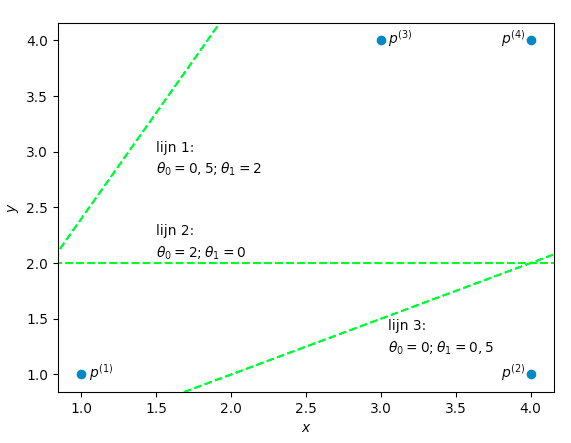
\includegraphics[width=.75\textwidth]{scatter4}
\caption{Een aantal mogelijke hypothese.\label{img:scatter4}}
\end{figure}

De vector $\theta$ beschrijft een hypothese van de verhouding tussen de gegeven en de gevraagde uitkomst. Voor elke observatie $x^{(i)}$ in de trainingsdata $X$ wordt aan de hand van $\theta$ de waarde van $h_\theta(x^{(i)})$ bepaald. Deze waarde wordt vergeleken met de \textit{actuele} waarde $y^{(i)})$. Het verschil tussen deze twee wordt gekwadrateerd en al deze verschillen worden bij elkaar opgeteld en gedeeld door het aantal samples om de gemiddelde kosten te krijgen die de huidige hypothese met zich meebrengt. Deze kosten worden weergegeven met $J$, wat dus een een functie is van $\theta$. De complete formule van de kostenfunctie is dus:

\[
J(\theta) = \frac{1}{2m}\sum_{i=1}^m(h_\theta(x^{(i)})-y^{(i)})^2.
\]

(De factor $2$ voor de $m$ mag je negeren, of je leest deze \href{https://math.stackexchange.com/questions/884887/why-divide-by-2m}{link}.)

\subsection{Lineaire regressie}

Het doel van lineaire regressie is de totale kosten $J(\theta)$ te minimaliseren: hoe lager deze waarde, hoe beter immers de hypothese overeenkomt met de werkelijke data. De algemene werking van \textit{lineaire regressie} staat in figuur \ref{img:overzicht} schematisch afgebeeld. Op basis van een dataset gebruiken we een leer-algoritme om een hypothese te formuleren over de verhouding tussen de gegeven en de gevraagde data. Op basis van deze hypothese kunnen we op basis van \textit{nieuwe} input (het woonoppervlak van een nieuwe aangeboden huis in Groningen) een voorstelling doen van de verwachte \textit{output} (de verwachte verkoopwaarde). Hoe beter de hypothese de gegeven data beschrijft, hoe beter de voorspellende waarde hiervan (hoewel hier ook wel een optimum aan zit; daar komen we later over te spreken wanneer we het gaan hebben over \textit{overfitting}).

\begin{figure}[h]
\centering
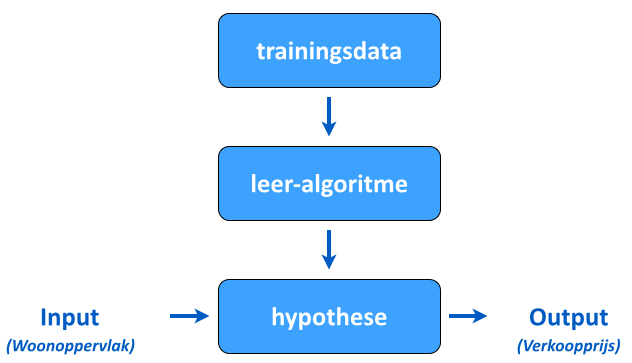
\includegraphics[width=.75\textwidth]{overzicht}
\caption{Lineaire regressie.\label{img:overzicht}}
\end{figure}

De vraag die dus voorligt is dus welke waarden de vector $\theta$ moet bevatten om $J(\theta)$ zo klein mogelijk te maken. Wanneer we ons voor het gemak even houden bij het huizenvoorbeeld van hierboven, wordt de vraag welke waarden $\theta_1$ en $\theta_2$ moeten hebben om de lijn de definiëren die het beste voorspelling van de prijs doet op basis van de grootte van het huis. Het algoritme dat hiervoor bestaat is betrekkelijk eenvoudig: kies een waarde voor $\theta_1$ en $\theta_2$, bereken $J(\theta)$ voor deze waarden en verander $\theta_1$ en $\theta_2$ zodat $J(\theta)$ kleiner wordt. Het probleem is natuurlijk hoe we deze veranderingen uit moeten rekenen.

In het huizenvoorbeeld wordt de hypothese van de prijs van een huis gedefinieerd door $h_{\theta}(x) = \theta_1 + \theta_2x$, waarbij $x$ de grootte van het huis is kwestie is. Op basis van de kostenfunctie, kunnen we een plot tekenen van $J(\theta)$ voor een grote \textit{range} van $\theta$. Omdat we twee variabelen hebben, wordt dit een driedimensionaal figuur zoals in figuur \ref{img:contour1}.

\begin{figure}[h]
\centering
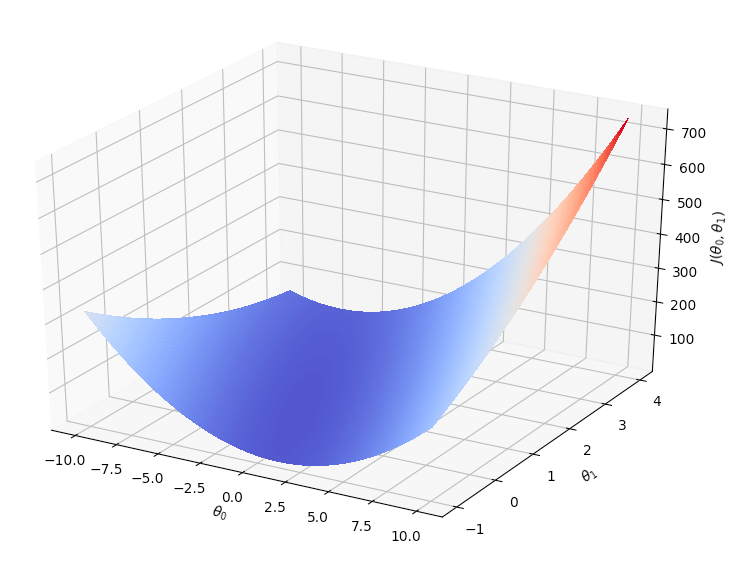
\includegraphics[width=.75\textwidth]{contour1}
\caption{Contour plot van drie dimensies.\label{img:contour1}}
\end{figure}

Voor elke waarde van $\theta$ kunnen we dus de hoek van de plot op dat punt bepalen, en die hoek kunnen we gebruiken voor onze update. We weten dat de hoek van een functie op een bepaald punt gegeven wordt door de \textit{afgeleide} van die functie te nemen. Dat geldt ook voor een functie die afhankelijk is van twee (of meer) variabelen, alleen moeten we in dat geval werken met de \textit{partiële} afgeleide. Wanneer we de snelheid van het algoritme weergeven als $\alpha$, dan wordt het algoritme dat we moeten uitwerken als volgt (zie appendix A voor het bewijs van deze partiële afgeleide):

\[
\begin{aligned}
&\textrm{Herhaal tot een minimum is bereikt} \\
& \textrm{(voor j=0 en j=1)} \{ \\
& \qquad\theta_j := \theta_j - \alpha \frac{\partial}{\partial\theta_j}J(\theta_0, \theta_1)\\
&\} 
\end{aligned}
\]



Van belang is dat je in dit stappenplan alle waarden van $j$ tegelijkertijd update. Dus je rekent eerst alle waarden uit en doet dan in één keer de update – anders krijg je een doorrekening van halve $\theta$'s. Omdat we meestal met meer dan één eigenschap (\textit{feature}) van de data te maken hebben, is het gebruikelijker (en makkelijker) om elke data-vector uit te breiden met een extra 1 aan het begin, zodat de dimensionaliteit van $\theta$ en van de data aan elkaar gelijk wordt – $\theta_0$ wordt dan eenvoudig vermenigvuldigd met die extra 1. Aldus uitgebreid en veralgemeniseerd, wordt het algoritme voor lineaire regressie

\[
\begin{aligned}
& \textrm{Herhaal tot een minimum is bereikt}\\
& \textrm{(gelijktijdige update voor alle $\theta_j$, $j=0 \hdots n$)}\{\\
& \theta_j := \theta_j - \alpha \frac{\partial}{{\partial}{\theta_j}}J(\theta) \\
& := \theta_j - \alpha \frac{1}{m}\sum_{i=1}^{m} (h_\theta(x^{(i)}) - y^{(i)})x_j^{(i)}\\
&\} .
\end{aligned}
\]

